\chapter{Le chiisme : histoire et doctrines}

\mn{21/3/22}
\section{bibliographie}
 

\begin{quote}
AMIR-MOEZZI, M-A. \emph{La religion discrète : croyances et pratiques
spirituelles dans l'Islam shi'ite}, Vrin, Paris, 2006.

AMIR-MOEZZI, M-A. et JAMBET, Christian \emph{Qu'est-ce que le shî'isme
?}, Fayard, Paris, 2004.

CORBIN, Henry \emph{En islam iranien: aspects spirituels et
philosophiques,} 4 volumes, Gallimard, Paris, 1991.

HALM, Heinz \emph{Le Chiisme}, Paris, PUF, 1995.

RICHARD, Yann \emph{L'islam chi'ite : croyances et idéologies}, Fayard,
Paris, 1991.

*TABATABA'I, Muhammad Huseyn \emph{Le chiisme en islam}, Beyrouth,
Al-Bouraq, 2009.
\end{quote}


\section{Le chiisme dans l'histoire
  musulmane. Quelques grands
  repères.}
  \label{le-chiisme-dans-lhistoire-musulmane.-quelques-grands-repuxe8res.}

On aurait pu traiter le développement du Chiisme et du sunnisme car ils ne se développent pas en vase clos. Mais il y a de tels différences,  en particulier, il n'y a pas de \textsc{foisonnement des visions dans le chiisme} du fait de l'importance des clercs
  

 \subsection{La naissance du chiisme : un problème de succession}
 ALi est le gendre et cousin du Prophète.
 
 Ali gagne à sa cause les nouveaux convertis (Egypte, Irak,...) et deviennent partisans d'Ali. Lorsque le Usman est assassiné en 656, Ali est élu comme 4ème calife. 
 \begin{Def}[ahl al-bayt]
\emph{famille du Prophète (Mahomet, Ali, Fatima, Hasan,
Hoseyn)}
 \end{Def}
 
 \paragraph{Mu'awiyya }Mais il est contesté par Mu'awiyya, qui lui reproche de ne pas chercher le meurtrier de Osman. En 657, bataille de Siffin, où les deux parties du monde arabe s'affrontent. Les Khalijites sont ceux qui reprochent à Ali d'avoir accepté l'arbitrage qui suit la bataille de Siffin.
 Ali est assassiné. Le califat est récupéré par Mu'awiyya.
 
 \paragraph{fondation de la dynastie des Omeyyades} par Mu'awyya. Hussayn, second fils de Ali s'oppose à Mu'awyya et est massacré dans la \textsc{plaine de Kerbala} avec sa famille et ses partisans. C'est le traumatisme fondateur. Le 10ème jour (Ashoura) du mois de Muharram, on rappelle ce martyr.
 
 \paragraph{une mosaique de courants shiites autour de la succession de l'imam et sur sa nature}
 Aujourd'hui, il y a trois courants : 
 \begin{itemize}
     \item ismaeliens :  7 imams
     \item zaydites : reconnaissent 5 imams
     \item imamites ou duodécimains : reconnaissent 12 imams.
 \end{itemize}
 
 Le Mahdi\sn{le Mahdi est aussi présent dans le sunnisme mais on ne sait pas qui c'est. Moins d'attente} n'est pas mort, il est occulté mais selon les courants, ce n'est pas le même. 
 
 \begin{Def}[mahdi]
   \emph{« le voilé » : l'homme mystérieux qui viendra annoncer et
provoquer la fin des temps (= dernier imam (occulté) pour les chiites).}
 \end{Def}
 
 \paragraph{Vision eschatologique forte dans le chiisme} Lutte du dernier imams contre le Dajjal, équivalent de \textit{l'antéchrist.}. Cela donne un potentiel révolutionnaire, avec certaines personnes se proclamant \textit{mahdi}, avec un potentiel mobilisateur très puissant, généralement révolutionnaire, voulant renversé le pouvoir établi, avec une forte dimension de justice sociale.
 
 
 
 %-------------------------------------------------
 \subsection{ « Le siècle chiite » : Bouyides et Fatimides (Xe-XIe s)}
 
 
 \paragraph{Diffusion du Chiisme à la mort de Hussayn} Dans les classes pauvres. En Irak par exemple, une grande révolte au IX ème siècle, se réclamant du chiime
 
 \paragraph{les bouyides} dans l'empire Abassides au X-XI, les Bouyides utilisent la faiblesse du calife pour s'imposer comme vizir, qui concentre la réalité du pouvoir : de 975, pendant environ un siècle.  
 
 \begin{figure}
     \centering
 
     \sidecaption{Source: \emph{Historical Atlas of Islam}, Malise Ruthven \& Azim Nanji,
Harvard University Press, 2004, p. 42.}
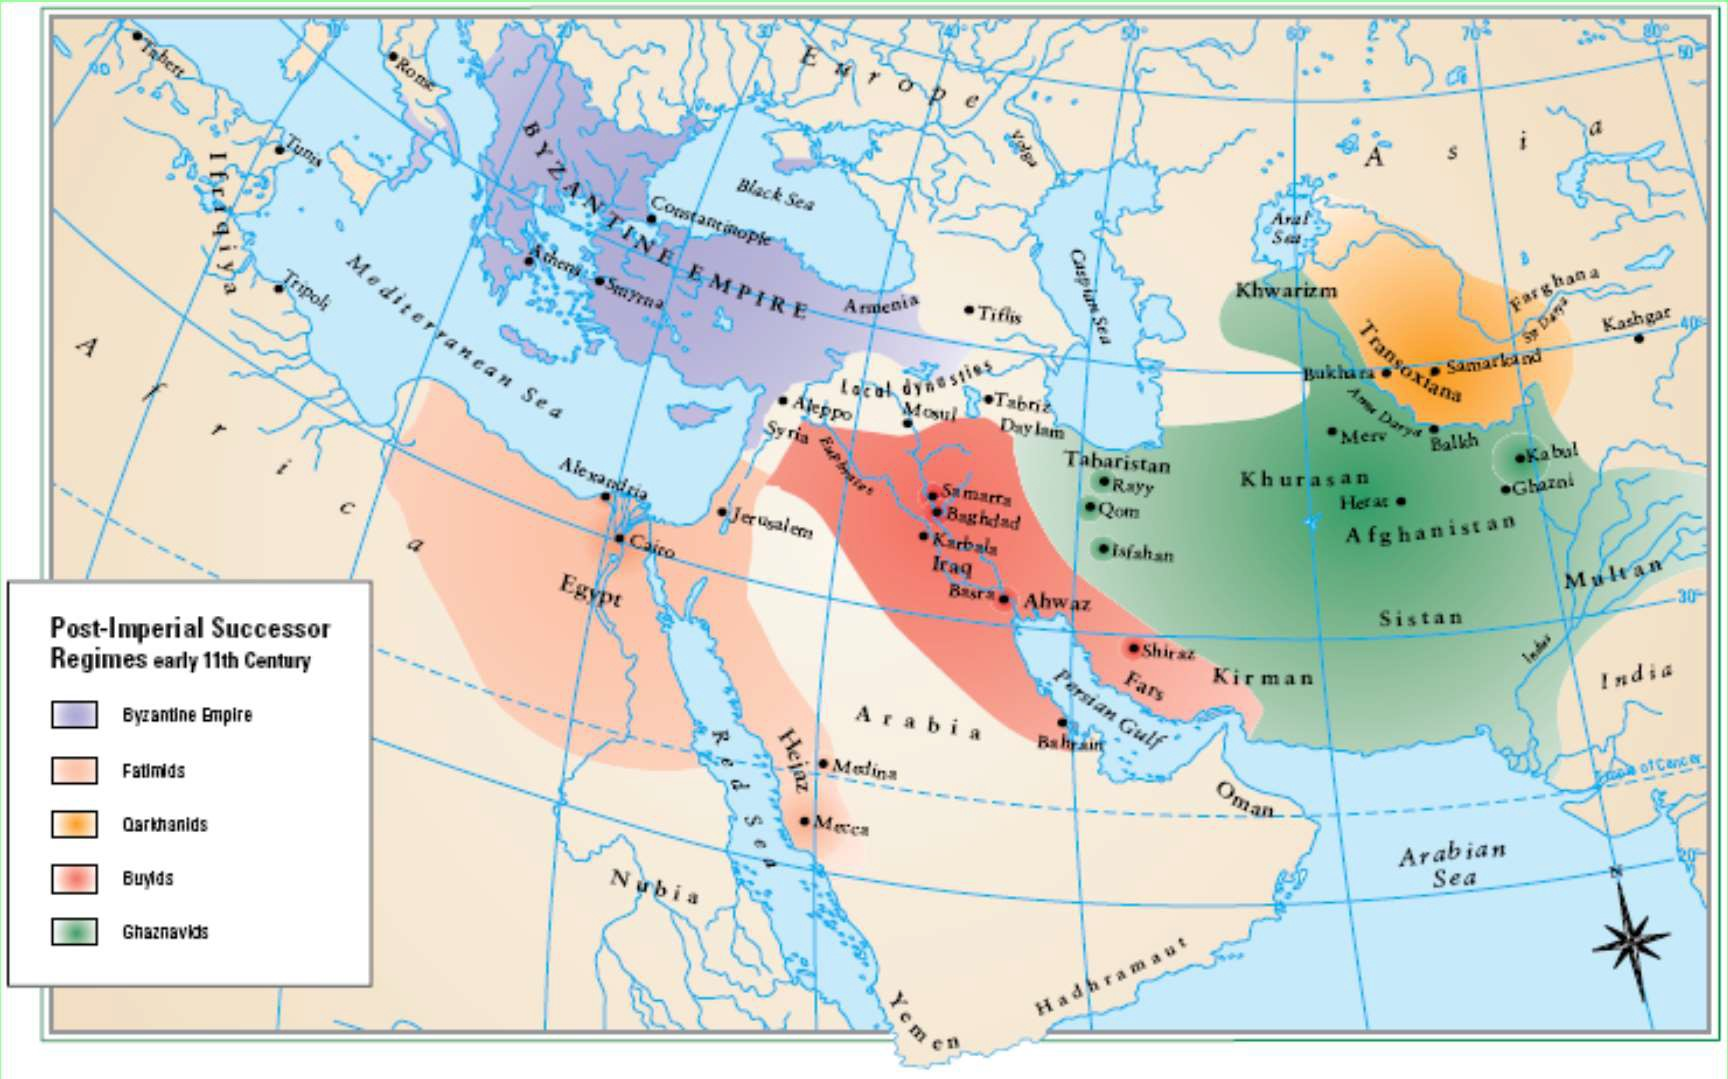
\includegraphics[width=\textwidth]{CourantsIslamContemporain/ImagesCourantsIslamContemporain/Image1Chiisme.jpeg}

     \label{fig:my_label}
 \end{figure}
 
 \paragraph{les fatimides} en afrique du Nord, fondé  par `Ubayd Allâh al-Mahdî (881-934). Typiquement, une personne se déclare Mahdi en Tunisie puis s'empare de l'Egypte (973 : le Caire comme capital). Avant le Caire n'était qu'une ville de garnison. 
 
 \paragraph{à Oman et au Yemen} AU Yémen, Zaydites, de 897 à 1962.
 
 
 %-------------------------------------------------
 
  \subsection{La naissance de l'Iran safavide (XVIe s.)}
 
  \begin{figure}
     \centering
 
     \sidecaption{Source: \emph{l'Iran safavide- Wikipedia}}
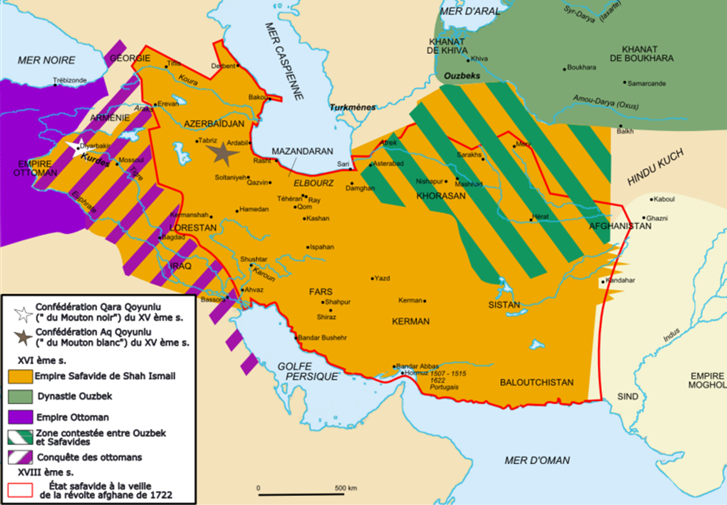
\includegraphics[width=\textwidth]{CourantsIslamContemporain/ImagesCourantsIslamContemporain/image2Chiisme.png}

     \label{fig:my_label}
 \end{figure}
 L'Iran était majoritairement sunnite jusqu'au Xème siècle. On a des populations turcophones à l'Ouest. un homme se proclame le Mahdi et fait la conquète militaire de l'Iran : par Isma'il en 1501.
  
 \paragraph{les limites du chiisme de Isma'il} conscient des limites du chiisme qu'il prone, il impose le chiisme duodécimain, venant du Liban, car le chiisme duodécimain était plus stable. Sans doute pour se détacher et légitimer face aux califes ottomans sunnites. Conversion de l'Iran assez violente : maudire les trois premiers califes, les confréries soufies. On va aussi déclarer les sunnites impurs.  


 
 %-------------------------------------------------
 
\section{Particularités de la doctrine chiite (duodécimaine ou imamite)
\label{particularituxe9s-de-la-doctrine-chiite-duoduxe9cimaine-ou-imamite}}


Elle s'est développée au VIII siècle par le 5ème et 6ème imams, qui étaient des savants. Ils ont collecté les corpus des hadiths, pas seulement du Prophète mais aussi des Imams, en particulier d'Ali et du 5ème et 6ème imams.

Ils ont développé l'école juridique
\begin{Def}[Ja'fariya]
 L'école juridique (madhhab) chiite dit Ja'fariya (aussi appelée école des Ahlul bayt) est la première école islamique apparue d'interprétation de fiqh du Coran d'inspiration chiite (contrairement aux quatre grandes écoles sunnites, avec lesquelles elle ne présente cependant pas de différences majeures).
\end{Def}
 %-------------------------------------------------
 
  \subsection{L'Imamat}
 La vraie spécificité du chiisme par rapport au sunnisme. 
 \begin{figure}[h!]
    \centering
        \sidecaption{lignée des imams}
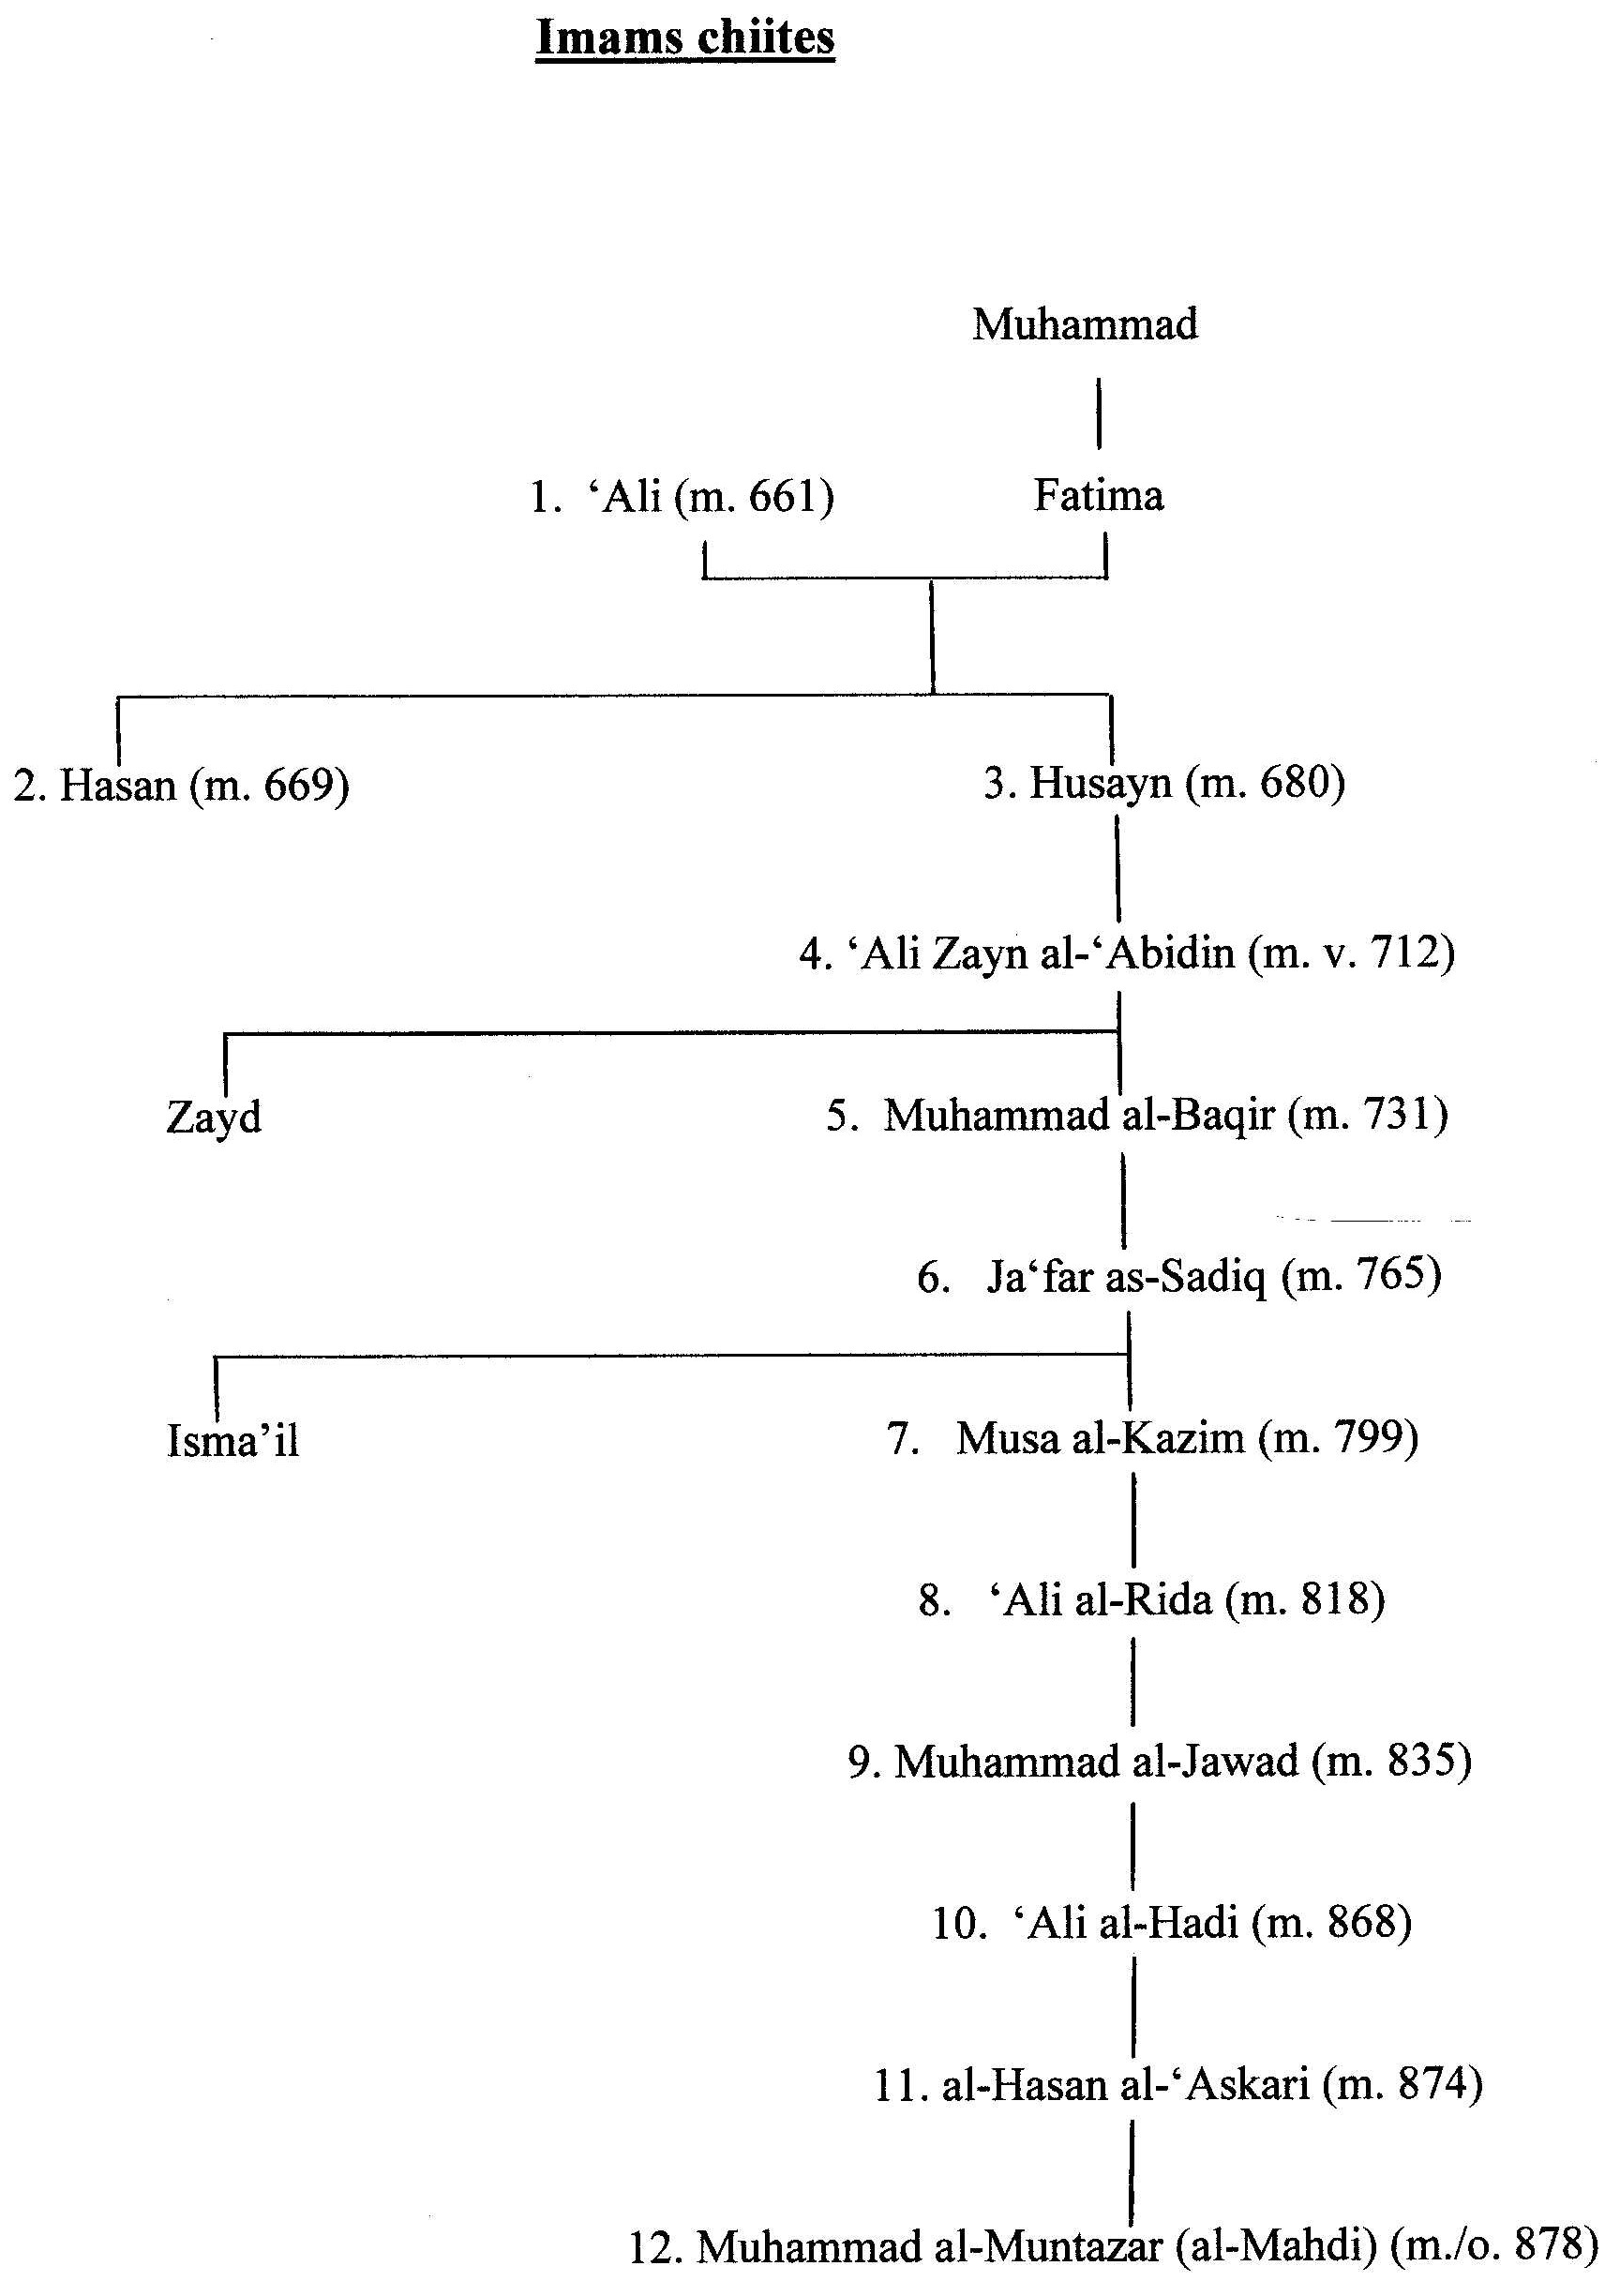
\includegraphics[width=0.8 \textwidth]{CourantsIslamContemporain/ImagesCourantsIslamContemporain/image2.png}
    \label{fig:my_label}
\end{figure}

 \paragraph{L'imam, celui qui guide} la prière et va faire le prêche du vendredi.  Dans la doctrine duodécimaine, l'imamat est lié à l'interprétation.
 Le prophète transmet la lettre du Texte. Mais elle a besoin d'être interprété : à chaque prophète dans l'humanité, correspond un imam : 
 \begin{itemize}
     \item Pour Moise, c'est Aaron
     \item Pour Jésus, c'est Pierre
     \item Pour Mohammad, c'est Ali.
 \end{itemize}
 Certes Mohammad est le dernier prophète, mais si on veut que le Coran soit parole vivante, il y a besoin d'Imams qui interprètent pour aujourd'hui la parole révélée.
 
 Du fait de problème de succession, il y a un vide à remplir (expliqué théologiquement par l'occultation), et c'est le \textit{clergé} qui le remplit \sn{Les Ayatollah ne sont pas imams. Il y a encore des imams dans le monde sunnite mais pas dans le monde chiite}.
 
 \newpage
 \paragraph{Les 14 immaculés}
    \begin{figure}
     \centering
     \sidecaption{Les 14 « Immaculés »  \newline La "Sainte Famille". \emph{Source}: Livre pour enfants iranien (Téhéran, 2006)}
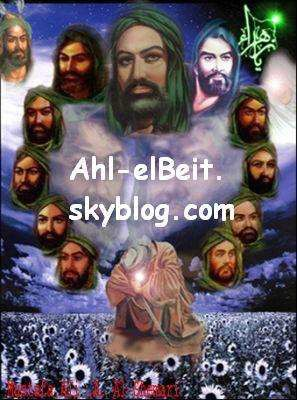
\includegraphics[width=0.45\textwidth]{CourantsIslamContemporain/ImagesCourantsIslamContemporain/Image3Chiisme.jpeg}
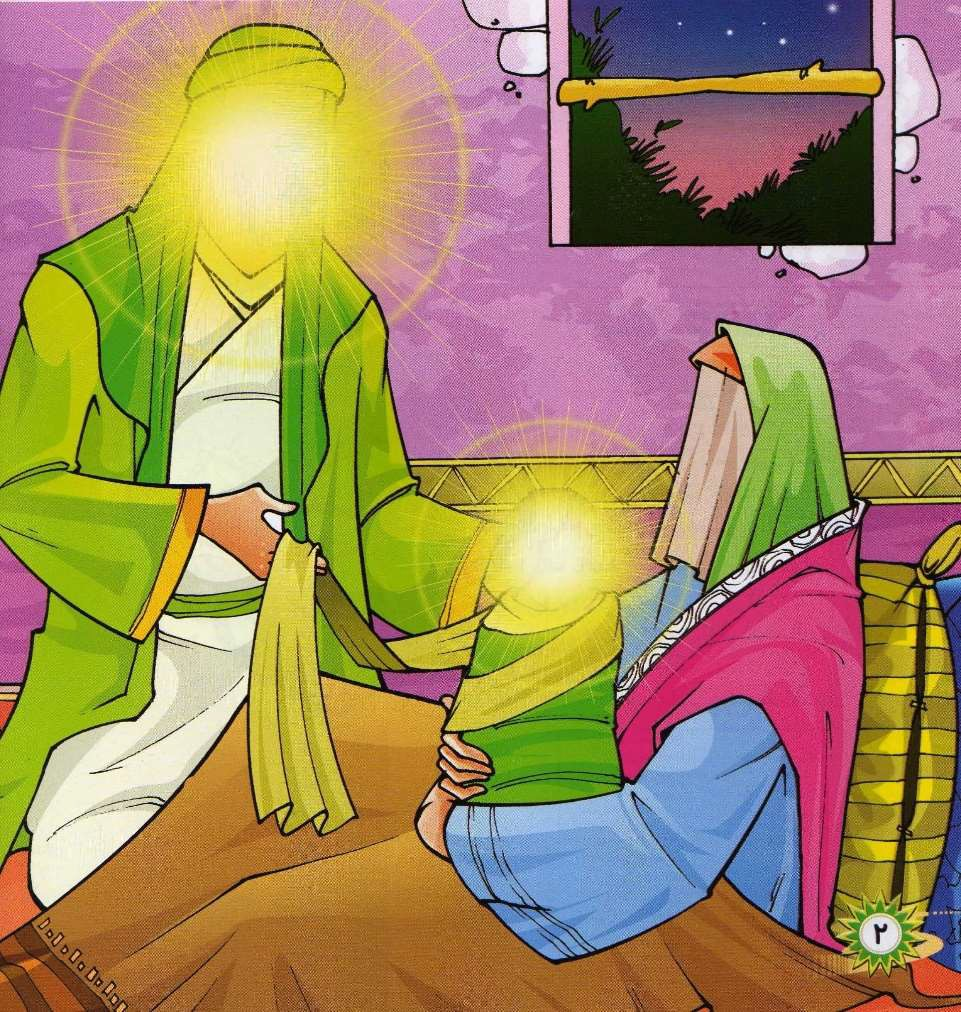
\includegraphics[width=0.45\textwidth]{CourantsIslamContemporain/ImagesCourantsIslamContemporain/image4.jpeg}
 \end{figure}
 
 
 \begin{Def}[les 14 immaculés]
 Les Quatorze immaculés ou Les Quatorze Infaillibles (en arabe:\TArabe{ المعصومون الأربعة عشر)} est l'expression désignant les gens de la Sainte Famille du Prophète Muhammad (s) Ahl al-Bayt, qui sont au nombre de quatorze, le premier étant le Prophète lui-même, suivi de sa fille Fâtima Zahrâ (a) et des douze Imams (a) qui lui ont succédé.
 \end{Def}
 
 
  
  
  \subparagraph{Prophétie et imamat}
  
 
Une autre tradition savante rapporte :\sn{(Source : \emph{La religion discrète}, M-A Amir Moezzi, Paris, Vrin,
2006, p. 110)}
\begin{quote}
    

« Deux mille ans avant la création, Muhammad et Ali étaient une lumière
devant Dieu -- qu'Il soit glorifié et exalté -, lumière formée d'un
tronc principal d'où partait un rayon de lumière resplendissant\ldots{}
Dieu dit alors : « Voici une lumière {[}tirée{]} de Ma propre Lumière ;
son tronc est la prophétie et sa branche, l'imamat ; la prophétie
revient à Muhammad, Mon serviteur et messager, et l'imamat revient à
Ali, ma Preuve et mon Ami. Sans eux, je n'aurai rien créé de ma
création\ldots{} C'est pourquoi Ali répétait toujours : « Je proviens de
Muhammad {[}ou de Ahmad{]} comme une clarté provenant d'une
autre\ldots{} »
\end{quote}


 \paragraph{Une science divine} pour interpréter le Coran, il y a besoin d'une science divine. L'imam a reçu une dimension spirituelle, la \textit{lumière de l'imamat}. Les imams préexistait à la création du monde en tant que réalité spirituelle. Comme les prophètes, ils sont \textit{impeccables}, sans péché.
   \subparagraph{La divinité des Imams}
De nombreux hadiths des Imams soulignent leur caractère quasi-divin : \sn{Source : « Remarques sur la divinité de l'Imam », M-A Amir-Moezzi,
\emph{Studia Iranica}, n° 25, 1996, p. 193-216}


\begin{quote}


« Hommes ! Dieu créa Ses serviteurs afin que ceux-ci Le connaissent car
lorsqu'Ils le connaissent, ils L'adorent et se libèrent ainsi de
l'adoration de tout autre que Lui ». Un homme demande alors à l'imam : «
Qu'est-ce que la connaissance de Dieu ? » « C'est pour les gens de
chaque époque, la connaissance de l'imam {[}de cette époque{]} auquel
ils doivent obéissance » (Husayn ben `Ali)

« Dieu fit de nous Son œil parmi ses adorateurs, Sa Langue Parlante
parmi Ses créatures, Sa Main de bienveillance et de miséricorde étendue
au-dessus de Ses serviteurs, Sa face grâce à laquelle on se dirige vers
Lui, Son Seuil qui guide vers Lui, Son Trésor au ciel et sur la
terre\ldots C'est par notre acte d'adoration que Dieu est adoré, sans
nous, Dieu ne saurait être adoré » (Ja`far as-Sadiq)


\end{quote}
 \paragraph{Les 14 impeccables} Le prophète, les 12 imams et Fatima. \sn{pas de difficulté de représentations dans le chiisme, depuis les enluminures persanes jusqu'à aujourd'hui. }
 
 \paragraph{le sacrifice d'Hussayn}
 
{Le martyre de l'imam Husayn}

Dans ce contexte, le martyre de Husayn, 3\textsuperscript{ème} imam, est
interprété dans les termes d'un sacrifice cosmique \sn{Source : tradition orale relevée par A-S Vivier-Muresan : \emph{Afzâd.
Ethnologie d'un village d'Iran}, Peeters, 2006, p. 48.
}:

\begin{quote}
    
 
Avant que le monde ne soit, Dieu rassembla les âmes des Quatorze
Immaculés, déjà créées, en une grande assemblée et leur annonça que,
pour ce monde qu'Il était sur le point de façonner, « du sang doit être
donné, un nourrisson et un tout jeune marié tués, une jeune femme
emprisonnée ». Aucun n'eut la force d'accepter de telles souffrances, ni
même Muhammad, ni Ali, ni Hasan. Seul Hoseyn se porta volontaire. Dieu
insista :
 

\begin{itemize}
\item
 
  Tu devras donner les tiens.
  
\item
  
  J'accepte.
  
\item
 
  Tu devras donner ta tête.
  
\item
 
  J'accepte.
  
\item
  
  Une partie de ta famille devra connaître l'exil et la détention.
  
\item
 
  J'accepte.
  
\end{itemize}


Alors Gabriel lui donna à boire la coupe de la souffrance et lui fit
signer un pacte où étaient inscrites toutes ses promesses.

Bien plus tard, lors de sa vie terrestre, approcha le temps de son
sacrifice. Il se trouvait à Karbalâ, accompagné de 72 fidèles compagnons
et de toute sa famille, encerclé par les armées de Yazid. Une armée de
djinns vint alors proposer ses services mais Hoseyn refusa : le combat
aurait été trop inégal et il se rappelait par ailleurs sa promesse. La
lutte commença et de nombreux êtres chers à Hoseyn, compagnons, fils,
frères, cousins, tombèrent l'un après l'autre sous les coups de
l'ennemi. Aveuglé par la douleur, Hoseyn en oublia sa promesse, et se
mit à tailler en morceaux l'armée adverse. Dieu s'empressa alors
d'envoyer Gabriel lui tendre le pacte qu'il avait signé au début des
temps. Rappelé à la raison, Hoseyn se soumit à la volonté divine et tint
son serment ; il retira son épée du combat et se livra à la fureur de
ses adversaires qui ne tardèrent pas à le mettre en pièces.
\end{quote}

 \subparagraph{Kerbala} la mémoire de la bataille est aussi une fête populaire. Des maquettes, repas,... le rouge reflète les partisans d'Hussayn.
 
 \begin{Def}[ta'ziyya]
\emph{représentation théâtrale du drame de Kerbala}
 \end{Def}

\begin{figure}[h!]
    \centering
        \sidecaption{Karbala}
    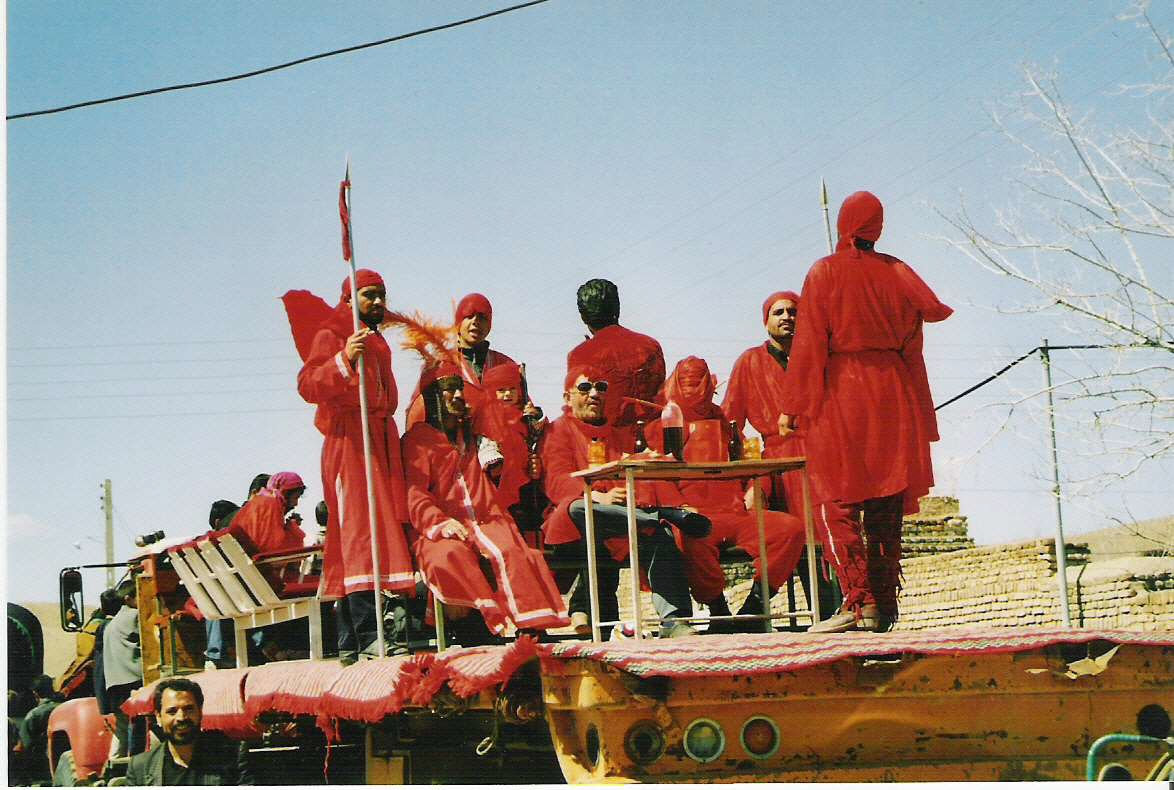
\includegraphics[width=0.3\textwidth]{CourantsIslamContemporain/ImagesCourantsIslamContemporain/image9.jpeg}
    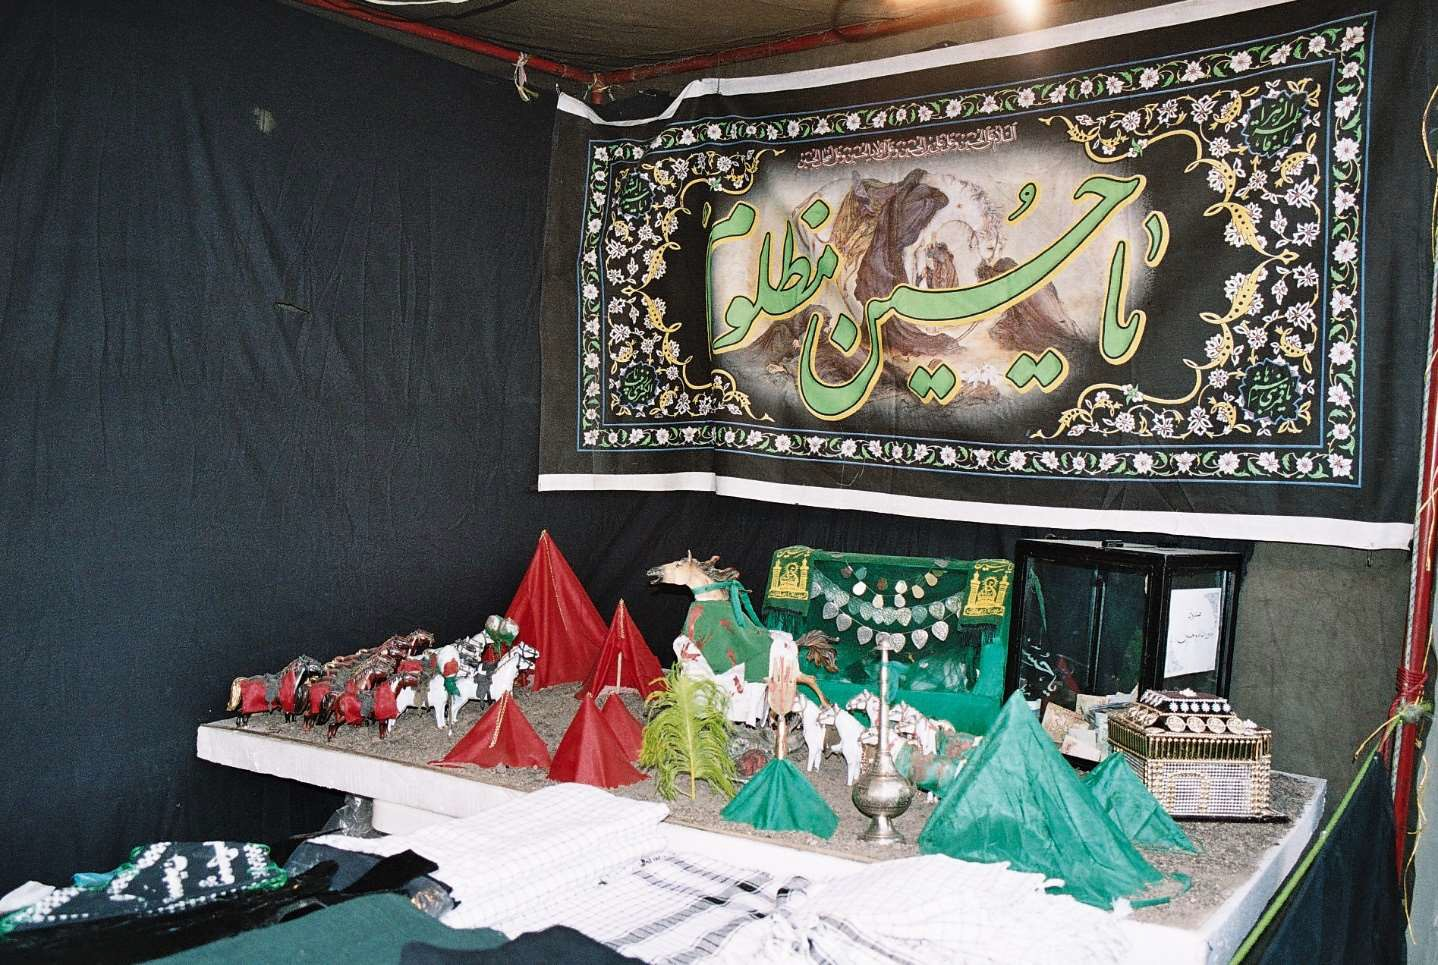
\includegraphics[width=0.3\textwidth]{CourantsIslamContemporain/ImagesCourantsIslamContemporain/image10Chiisme.jpeg}
        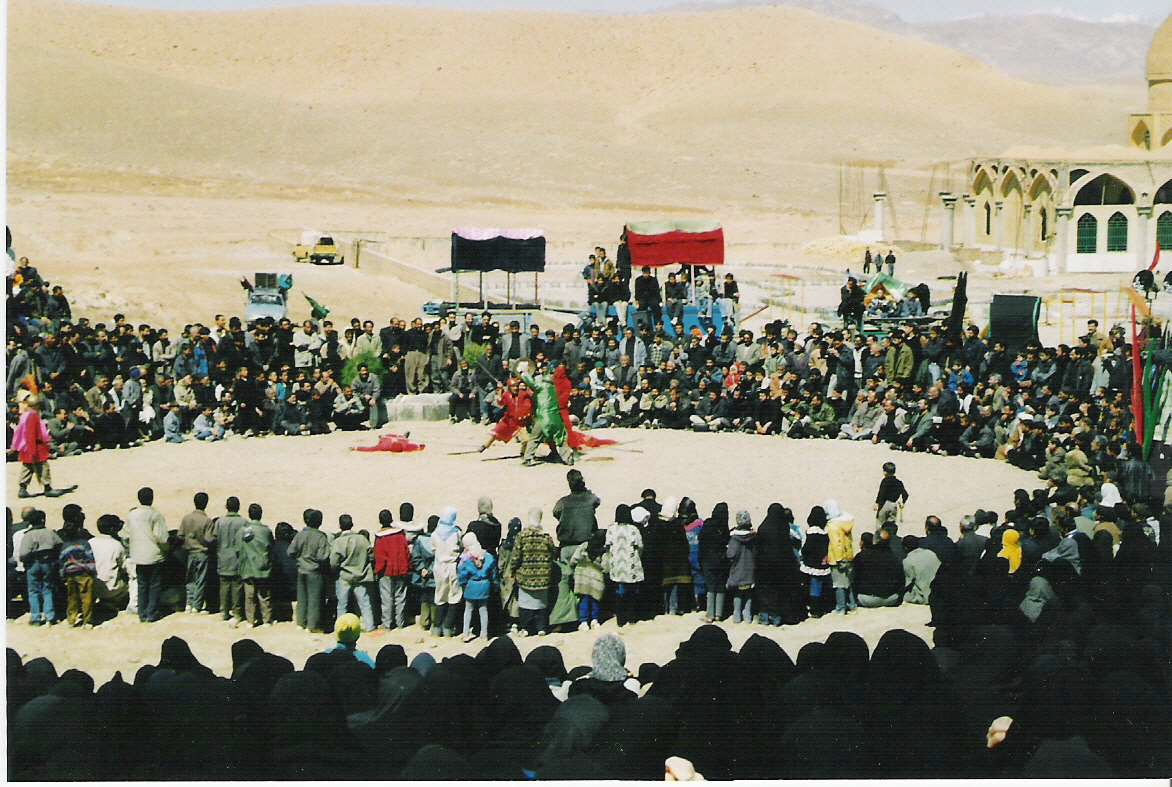
\includegraphics[width=0.3\textwidth]{CourantsIslamContemporain/ImagesCourantsIslamContemporain/image8.jpeg}


    \label{fig:my_label}
\end{figure}
 
 
 %-------------------------------------------------
 
  \subsection{Le corpus coranique et son interprétation}
 
 
  \paragraph{Le « Coran chiite »}
 
 Le Coran actuel aurait été purgé des 2/3, en particulier par tout ce qui touche 'Ali.


\begin{quote}
Certains écrits chiites rapportent des citations du «Coran intégral»
qui aurait été par la suite altéré par les sunnites. Ces citations
présentent des divergences parfois notables avec la recension
officielle, comportant souvent des mots, expressions ou bouts de phrase
absents de celle-ci (en italique dans le texte).

C. 4, 167-70 : « Ceux qui sont injustes \emph{à l'égard des droits de la
Famille de Muhammad}, Dieu ne les pardonnera ni ne les guidera sur aucun
chemin si ce n'est sur celui de la géhenne où ils y séjourneront à
jamais et c'est chose facile à Dieu.

C. 16, 24 : « Et quand on leur dit : `\,`Qu'a fait descendre votre
Seigneur \emph{au sujet de `Ali} ?'\,' Ils répondent : `\,`Fables
racontées par les Anciens'\,' » ?

C. 33, 71 : « Quiconque obéit à Dieu et à Son prophète \emph{en ce qui
concerne la walaya de `Ali et la walaya des imams après lui}, celui-là
jouit d'un bonheur grandiose ».

C. 42, 13 : « Il a établi pour vous, \emph{ô famille de Muhammad}, en
fait de religion, ce qu'Il avait prescrit à Noé, et ce que Nous te
révélons \emph{ô Muhammad}, et ce que Nous avons prescrit à Abraham, à
Moïse et à Jésus : `\,`Etablissez la religion \emph{de la famille de
Muhammad}, ne vous divisez pas à son sujet et soyez unis ».

(Source : \emph{La religion discrète}, M.A Amir-Moezzi, Paris, Vrin,
2006, p. 179-180)
\end{quote}
 
 A la fin du XIX, cette posture chiite a été abandonnée car le réformiste chiite a essayé de se rapprocher du sunnisme. De façon générale, le Coran lu en Iran a toujours été le même mais avec une suspiçion qu'il ne contenait pas tout.
 

 %-------------------------------------------------
 
  \subsection{Le rôle des clercs}
  
  \paragraph{Un sens caché du Coran, ésotérique} Seul l'imam peut interprété le Coran. \textit{"si le grand ayatolah nous dit qu'on ne doit plus prier 5 fois par jour, on le suit".} \sn{L'absence de médiation dans le sunnisme est à relativiser quand on voit l'importance pour les sunnites de ce qui est Halah et Haram et qui demandent à l'imam...}
 
 \paragraph{Les clercs vont se substituer à l'Imam} pour l'interprétation du Coran et du droit. 
 
 \paragraph{Direction de la prière} A l'époque safavide, le clerc est nécessaire pour diriger la prière. On ne peut prier collectivement sans clerc. Le clerc va s'occuper des taxes religieuses.
 \paragraph{Au XIX, déclaration du Jihaad} Alors que c'est normalement l'Imam.
 
 \paragraph{Une dernière étape, avec l'Ayatollah Khomeini, le pouvoir politique} Toutes les prérogatives normalement réservées à l'Imam.
 
 \paragraph{Un clergé très structuré}. 
 \begin{itemize}
     \item les \emph{marja} (taqlid), la \emph{source} (de l'imitation). Un fidèle doit imiter un marja. Une dizaine dans le monde. Ils se cooptent (des dynasties de Marja et d'ayyatollah). Khomeini était \textit{marja}.
     \item l'\emph{ayyatollah} qui est le seul à interpréter le Coran, une centaine dans le monde, dont quelques femmes
     \item le \emph{hojjatelislam} qui a l'équivalent d'un doctorat
     \item le \emph{mollah}, \emph{âkhund} qui dirige la prière
 \end{itemize}
 
 
 %-------------------------------------------------
 
  \section{D'autres courants chiites :
  Zaydites et
  Ismaéliens} 
 
   \subsection{Le zaydisme}
   
   Proche du sunnisme, ils reconnaissent même les trois premiers califes, ce qui est inconcevable dans le chiisme duodécimain (cf la cérémonie de bruler Omar de Khomeini).
   Environ 1 million de fidèle.
   
   \subsection{Le chiisme septimain (ismaélisme)}
   A l'autre extrême, l'imam est quasiment une incarnation de Dieu. Un primat de l'ésoterisme, occulte. Un grand rôle donné à l'initiation. Un certain recul par rapport aux pratiques, à relativiser. 

\paragraph{L'Aga Khan} chef spirituel des septimains.
 



 
\section{Glossaire}
 
\subsection{Personnes} Abbas Abu Bakr

Adud ad-Dawla Al-Karaki Hasan as-Sabah Isma'il

Kulayni (\emph{Kitab al-Kafi}) Mu'awiya (omeyyades) Nizar

Omar Osman Quraysh Yazid

{Lieux} Alamut Ardabil

Ghadir al-Khumm Jabal al-Amil Kerbala

Khorasan Kufa Machhad Sham Siffin

{Autres noms propres} akhbari

ja`farisme (école juridique chiite) kharijites

Mamlouks

Muharram (mois musulman) mu`tazilites

nizayri Qarmates Seljukides usuli

\subsection{Notions}



baten : \emph{ésotérique} (c. zaher) faqih (pl. fuqaha) : \emph{juriste}

fitna: \emph{discorde, querelle (conflit interne au monde musulman)}

ghulat : \emph{groupes chiites aux doctrines}

\emph{« extrémistes »}

hulul : \emph{« incarnation »}

ijtihad : \emph{effort personnel d'interprétation (des textes sacrés)}

`ilm : \emph{science}

imamzade : \emph{descendant des Imams / sanctuaire contenant leur
tombeau} (persan)

`isma : \emph{impeccabilité}



ma`sum : \emph{impeccable (sans péché)} mujtahid : \emph{celui qui
pratique l'ijtihad} najes : \emph{impur} (persan)

na'ib : \emph{délégué}

na'ib al-`amm : \emph{représentant général de l'Imam}

nass : \emph{élection divine}

tafsir : \emph{commentaire (exotérique) du Coran}

tanasukh : \emph{métempsychose}

ta'wil : \emph{herméneutique ésotérique du Coran} 


taqiyya : \emph{dissimulation (fait de cacher sa foi)} walayat al-faqih
(persan : velayat-e faqih) : \emph{gouvernement du juriste}

zaher : \emph{exotérique} (c. de baten)
 
 


 



 


 